\documentclass{beamer}
\usepackage{beamerthemesplit}
\usepackage{graphicx,url}
\usepackage[brazil]{babel}
\usepackage[utf8]{inputenc}
\usepackage{multimedia}

\mode<presentation>
{
  \usetheme{Ilmenau}
  \setbeamercovered{transparent}
}

\newcommand{\eng}[1]{\textit{#1}}
\newcommand{\obra}{\textit{Em torno da romã}}
\newcommand{\goiaba}{\textit{Goiaba}}
\newcommand{\redmark}[1]{\textcolor{red}{#1}}
\newcommand{\graymark}[1]{\textcolor{gray}{#1}}
\newcommand{\tocar}{\textcolor{blue}{$\blacktriangleright$}}

\title{Goiaba}
\author{Marcos S. Sampaio e Pedro Kröger}
\date{28 de novembro de 2008}

\logo{
\includegraphics[scale=.15]{logo-genos}}

\begin{document}

\frame{\titlepage}

\section{Contornos}

\frame{
  \frametitle{Contornos em Música}
  \begin{figure}
    \centering
    \includegraphics{5a-sinfonia}
  \end{figure}

  \href{run:audio/5a-sinfonia.ogg}{\tocar}

  \begin{figure}
    \centering
    \includegraphics[scale=1.4]{c-3120-simples}
  \end{figure}
}

\frame{
  \frametitle{Semelhança e possível coerência}
  \begin{figure}
    \centering
    \includegraphics{ly-3120-qualquer}
    \hspace{1em}
    \includegraphics[scale=1.4]{c-3120-simples}
  \end{figure}
  \vspace{-1em}

  \href{run:audio/ly-3120-5a-sinfonia.ogg}{\tocar}
}

\frame{
  \frametitle{Pontos positivos}
  \begin{itemize}
  \item Possível coerência
  \item Manipulação por operações \cite{morris87:composition,friedmann85:methodology,adams76:melodic}
  \item Representação gráfica
  \end{itemize}
}

\frame{
  \frametitle{Operações}
  \begin{itemize}
  \item implementadas no \goiaba{} (rodar no programa)
  \end{itemize}
}

\section{Composição}

\frame{
  \frametitle{Rotação com retrogradação}
  \begin{figure}
    \centering
    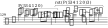
\includegraphics[scale=2.5]{sujeito-fugato}

    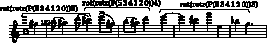
\includegraphics[scale=2.5]{contra-sujeito-fugato}
  \end{figure}

  \href{run:audio/fugato.ogg}{\tocar}
  \tiny (mostrar operações no \goiaba{})
}


\section{Conclusões}

\frame{
  \frametitle{Trabalhos futuros}
  \begin{itemize}
  \item Implementação de mais funções
  \item Lançamento de uma versão para usuário
  \item Interface gráfica
  \item Api fácil de usar
  \item Conversão de/para partituras musicais
  \end{itemize}

  \tiny
  O Goiaba está disponível em \url{wiki.genos.mus.br/goiaba}
}

\renewcommand{\refname}{Referências}

\bibliographystyle{apalike}
\bibliography{melodic-contour}

\end{document}
